\section{Method}

Recall that our objective is to, given a rank $D$ matrix $\mathcal X \in \mathbb R^{D \times P}$ with $P > D$, select a square submatrix $\mathcal X_{.\mathcal S}$ where subset $\mathcal S \subset P$ satisfies $|\mathcal S| = D$ that is as unitary as possible.
Thus, we first will define a function that is uniquely minimized by unitary matrices and some favorable properties for optimization that will be the ground truth we evaluate the success of our method against.
We then define the combination of normalization and multitask basis pursuit that approximates this ground truth loss function.
We include claims that ground truth and convex loss values are the same for all diagonalizable matrices, and that the convex basis pursuit program recovers to optimum in a deterministic manner should it exist; proofs are given in Section \ref{sec:proofs}.
% NOTE (Sam): we have not yet shown that the optimum is always D sparse if it exists... but this should be doable.
We finally define the lasso dual to the basis pursuit program and a post processing method for ensuring that the solution is $D$ sparse.
Experimental results using these methods will then be given in Section \ref{sec:experiments}

\subsection{Ground truth}
\label{sec:ground_truth}

The main goal of isometry pursuit is to expediate the selection of unitary submatrices.
More traditional measures of unitariness which use the singular values of a matrix like the log operator norm (i.e. log deformation) and nuclear norm are poorly suited for  optimization since they use a subset of the matrix's information and are not uniquely minimized at unitarity, respectively.
% NOTE (Sam): %is our the convex dual of itself?
Thus, we define the loss
\begin{align}
l_{c}: \mathbb R^{D \times P} \to \mathbb R^{+} \\
\mathcal X \mapsto \sum_{d = 1}^D g(\sigma^d(\mathcal X), c)
\end{align}
where $\sigma^d (\mathcal (X))$ is the $d$-th singular value of $\mathcal X$ and
\begin{align}
g: \mathbb R^+ \times \mathbb R^+ &\to \mathbb R^+ \\
t,c &\mapsto e^{t^c} + e^{t^{-c}}.
\end{align}
Plainly, $g$ is uniquely maximized by unitary matrices, and $g(\mathcal X^{\dagger}) = g(\mathcal X)^{-1}$.
The former condition is necessary for success of the method, while the latter, as well as the convexity of $g$, are somewhat aesthetic choices.
A graph of $g$ is given in Figure \ref{fig:gt_loss}.
Most importantly, this loss enables comparison with produced after normalization as in Section \ref{sec:normalization}.
%This loss is an appropriate choice for comparison because it is equal to the basis pursuit loss for suitably normalized orthogonal matrices.

% NOTE (Sam): this could be improved.  Do we need proofs of maximized by unitary matrices and convex?
% Something like the justification for logarithmic symmetry would be useful here.
% Why do we need convex here? Convex functions form metric? Cite Koelle neuroscience? Is metric important?
% Can we prove this is a norm?

The overall algorithm we seek to improve upon is 
\begin{align}
\label{prog:ground_truth}
\widehat {\mathcal S}_{GT}  &= \arg \min_{\mathcal S \subseteq [P] : |\mathcal S| = D} l_c (\mathcal X_{.\mathcal S})
\end{align}

In practice, non-convexity occurs in two places, but only one is essential.
The inessential non-convexity is in the computation of $l_c$.
While this function is in fact convex, computation of the individual singular values prior to summation is not, and our experiments rely on such piecemeal computation rather than implementing an end-to-end method.
% NOTE (Sam): add a citation and check this is convex
However, the combinatorial search over $[P]$ is inherently non-convex, and requires combinatorial search over all combinations.
% NOTE (Sam): check what this type of optimization problem is called.  Integer programming?  Is there a dynamic programming solution?

\subsection{Normalization}
\label{sec:normalization}
% NOTE (Sam): balance goes out the window with great flowers since there is no normalization.

% NOTE (Sam): it might be nice to borrow the normalization, optimization, and postprocessing step lexicon from the neuroscience paper.
We will propose a basis pursuit method which approximates the results of Program \ref{prog:ground_truth}.
Since basis pursuit methods tend to select longer vectors, selection of unitary submatrices requires normalization such that long and short candidate basis vectors are penalized in the subsequent regression.
This calls for a "normalization" method that differs from other forms in its requirements, and we can't yet prove that these conditions relate it to any sort of norm, even on an appropriately chosen space.
This normalization is 
Now establish some basic conditions for normalization of vectors $v \in \mathbb R^D$.

\begin{definition}[Symmetric normalization]
% NOTE (Sam): need a better name for this type of function.  Can I reuse parts in ground truth section?  Keep in mind max/min is switched).
A function $q: \mathbb R^D \to \mathbb R^+ $ is a symmetric normalization if 
\begin{align}
\arg \max_{v \in \mathbb R^D} \ q (v) &=\{ v : \|v\| = 1 \} \\
q(v) &= q(\frac{v}{\|v\|^2}) \\
q(v^1) &= q(v^2) \; \forall \; v^1, v^2 : \|v^1\| = \|v^2\|
\end{align}
\label{cond:normalization}
\end{definition}

Note that requiring the full structure of a multiplicative norm here is unnecessary for basic success of the algorithm, but certain characteristics such as $q(v^{-1}) = q(v)$ seem desirable, provided one can give a reasonable way to compute $v^{-1}$, such as by considering each vector as a scaled rotation subgroup of the general linear group.
Mindful of this opportunity, and also of the desire to compare with the ground truth and provide computational expediency, consider the normalization by
\begin{align}
\label{eq:normalization}
% Note (Sam): fix this... get and more ... q_c?
q: \mathbb R^+ \times \mathbb R^+  &\to \mathbb R^+ \\
t , c &\mapsto \frac{e^{t^c} + e^{t^{-c}}}{2e},
\end{align}
and use this to define the vector normalization 
\begin{align}
n: \mathbb R^D \times \mathbb R^+ &\to \mathbb R^D \\
n , c &\mapsto \frac{n}{q(\|n\|_{2},c) }
\end{align}
and matrix normalization
\begin{align}
w: \mathbb R^{D \times P} \times \mathbb R^+ &\to \mathbb R^D \\
\mathcal X_{.p} , c &\mapsto n(\mathcal X_{.p}, c) \; \forall \; p \in [P].
\end{align}

While this normalization satisfies \ref{cond:normalization}, it also has some additional nice properties.
First, $q$ is convex.
Second, it grows asymptotically log-linearly.
Third, while $\exp(-|\log t|) = \exp(-\max (t, 1/t))$ is a seemingly natural choice for normalization, it is non smooth, and the LogSumExp replacement of $\max (t, 1/t)$ with $ \log (\exp (t ) + \exp(1/t))$ simplifies to \ref{eq:normalization} upon exponentiation.
% Introduce the exponent here.
Finally, the parameter $c$ grants control over the width of the basin, which is important in avoiding numerical issues arising close to $0$ and $\infty$.
This completes the deterministic data preprocessing.

\begin{figure}[htbp]
% NOTE (Sam): need to figure out how to make these subfigures
    \centering
       \begin{minipage}{0.32\textwidth}
        \centering
        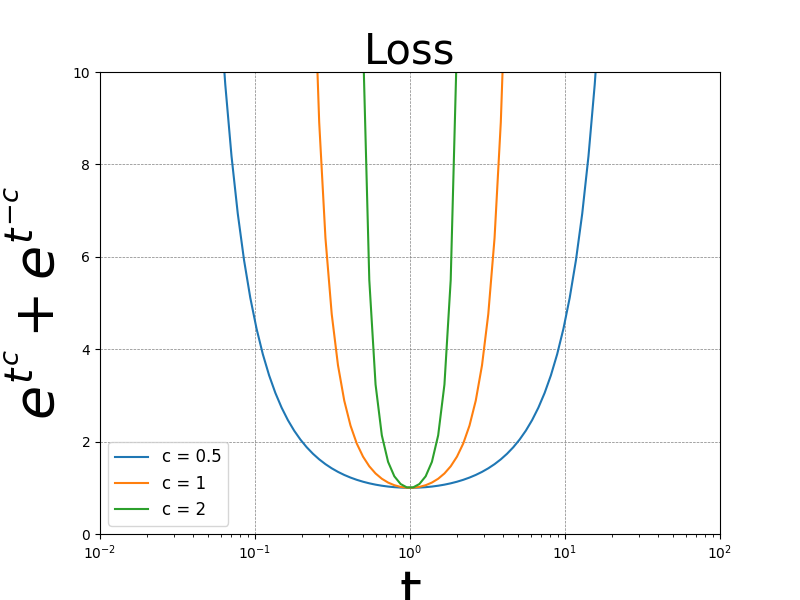
\includegraphics[width=\textwidth]{../figures/Figure_1b.png}
        \caption{Ground truth loss scaling function $g$ as a function of $t$}
        \label{fig:gt_loss}
    \end{minipage}
    \begin{minipage}{0.32\textwidth}
        \centering
        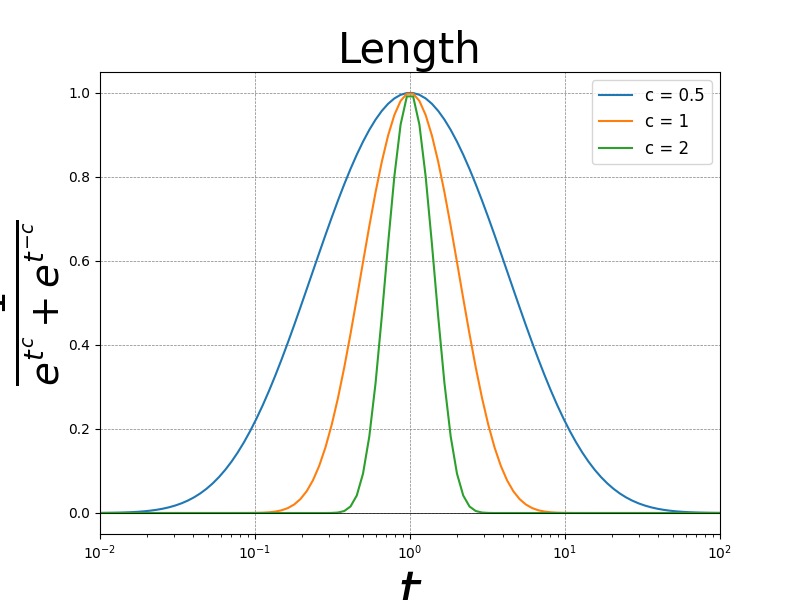
\includegraphics[width=\textwidth]{../figures/Figure_1a.png}
        \caption{Length as a function of $t$}
        \label{fig:length}
    \end{minipage}
    \begin{minipage}{0.32\textwidth}
        \centering
        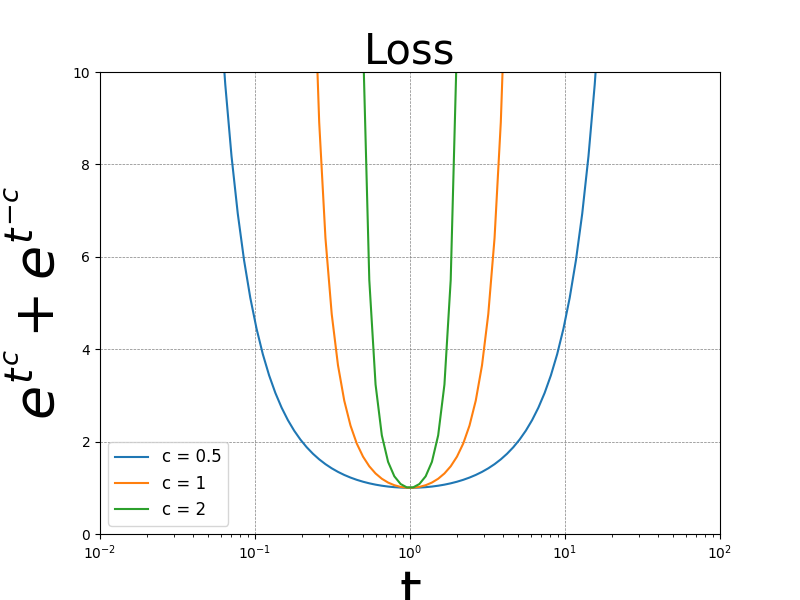
\includegraphics[width=\textwidth]{../figures/Figure_1b.png}
        \caption{Basis pursuit losses as a function of $t$}
        \label{fig:loss}
    \end{minipage}
    \caption{Plots of Length and Loss for different values of $c$.
    Since $t$ is one dimensional and therefore diagonalizable, basis pursuit and ground truth give identical loss values.}
    \label{fig:results}
\end{figure}

\subsection{Isometry pursuit}

We will show how to use an appropriate normalized matrix $w(\mathcal X)$ in multitask basis pursuit to identify submatrices of $\mathcal X$ that are as unitary as possible.
Multitask basis pursuit is a method for identifying sparse signals from overcomplete dictionaries, and the intuition behind its application in our setting is that submatrices consisting of vectors which are closer to 1 in length and more orthogonal will have smaller loss.
In contrast to the typical statistical setting, these features correspond to individual observations in our diversification example, and basis vectors of data manifold tangent spaces in our non-linear dimension reduction example.

Define the multitask basis pursuit penalty  % is this really a norm?
\begin{align}
\label{eq:bp}
\| \cdot \|_{1,2}: \mathbb R^{P \times D} &\to \mathbb R^+ \\ 
\beta &\mapsto  \sum_{p=1}^P  \|\beta_{p.}\|_2.
\end{align}
The isometry pursuit program is then
\begin{align}
\label{prog:isometry_pursuit}
\widehat \beta^{P}_c (\mathcal X)  := \arg \min_{\beta \in \mathbb R^{P \times D}} \| \beta \|_{1,2} \; : \; I_D = w ({ \mathcal X}, c) \beta.
\end{align}
The recovered functions are the indices of the dictionary elements with non-zero coefficients.
That is, they are given by $S(\beta)$ where 
\begin{align}
S: \mathbb{R}^{p \times d} &\to \binom{[P]}{d} \\
\beta &\mapsto \left\{ p \in [P] :  \|\beta_{p.}\| > 0 \right\}
\end{align}
and $\binom{[P]}{d} = \left\{ A \subseteq [P] : \left|A\right| = d \right\}$. 
\begin{algorithm}[H]
\caption{\isometrypursuit(Matrix $\mathcal X \in \mathbb R^{D\times P}$, scaling constant $c$)}
\begin{algorithmic}[1]
\STATE {\bf Output} $\widehat S= S (\widehat \beta_P(w_c(\mathcal X))$ 
\end{algorithmic}
\end{algorithm}

A key theoretical assertion for the feasibility of \isometrypursuit~ is that it is invariant to choice of basis for $\mathcal X$.
\begin{proposition}[Basis pursuit selection invariance]
\label{prop:basis_pursuit_selection_invariance}
Let $U \in \mathbb R^{D \times D}$ be unitary.
 Then $S(\widehat \beta  (U \mathcal X)) = S(\widehat \beta (\mathcal X))$.
\end{proposition}
A proof is given in Section \ref{proof:basis_pursuit_program_invariance}
This fact has as an immediate corollary that we may replace $I_D$ in the constraint by any unitary $D \times D$ matrix.

With these preliminaries, we may state our main result.
From an intuitive perspective, this is akin to saying selected columns are not only complementary in that they are orthogonal, but also well-balanced in that their columns are of a standard length.
\begin{proposition}[Unitary selection]
\label{prop:unitary_selection}
Given a matrix $\mathcal X \in \mathbb R^{D \times P}$ with a rank $D$ submatrix $\mathcal X_{.\mathcal S} \in \mathbb R^{D \times D}$ that is unitary, $\mathcal S = S(\widehat{\beta} (\mathcal X)))$
 \end{proposition}
 
This proof admits two immediate generalizations.
First, any normalization function that satisfies the normalization conditions will do.
Second, assuming that we do in fact use $w$ for normalization, the ground truth and convex losses are equivalent for diagonalizable matrices.
This is summarized in the following proposition, which is slightly stronger than Proposition \ref{prop:unitary_selection}
 \begin{proposition}[Loss equivalence]
 Given a diagonalizable matrix $\mathcal X \in \mathbb R^{D \times D}$, $\|\widehat \beta_c^P(\mathcal X)\|_{1,2} = l_c (\mathcal X)$.
 \end{proposition}
This proposition should be thought of as applying to $D$ column matrices after selection.
We know that unitary submatrices minimize loss, and should they be present, they will be selected by either method. % Note (Sam): still need to prove!
This proposition shows that should diagonalizable matrices be selected, they will also have equivalent loss, but not necessarily that they will be selected.
% NOTE (Sam) is it just generally required that q(v) = g^{-1} (\|v\|) v/\|v\| basically?  Might need to make normalization notation more clear to state general proposition.



\subsection{Isometric lasso}

The convex loss function \ref{eq:bp} and linear constraint in \ref{prog:isometry_pursuit} admit a Lagrangian dual which we shall call Isometric Lasso.
While we defer full discussion of computational complexity to Section \ref{sec:computational_complexity}, the general principal which motivates the use of this formulation in our setting is the increased computational expediency in high-dimensions.

The Isometric Lasso loss is
\begin{align}
l_\lambda (\mathcal X, \beta) =  \|I_D -  \tilde{ \mathcal X}_c \beta\|_2^2 +  \lambda \| \beta \|_{1,2}
\end{align}
which can be optimized as
\begin{align}
\label{prog:isometric_lasso}
\hat {\beta_{\lambda}} (\mathcal X) = \arg \min_{\beta \in \mathbb R^{P \times D}} l_\lambda (\mathcal X, \beta)
\end{align}

Similarly to Section \ref{sec:isometry_pursuit}, we assert that $S(\widehat {\beta}_{\lambda} (\mathcal X))$.

\begin{proposition}[Lasso selection equivalence]
\label{prop:lasso_selection_equivalence}
Let $U \in \mathbb R^{D \times D}$ be unitary.
 Then $S(\widehat \beta_{\lambda}  (U \mathcal X)) = S(\widehat \beta_{\lambda} (\mathcal X))$.
\end{proposition}

This also covers changing the target variable.

Note that it also may be possible to argue the basis pursuit invariance from the lasso ones plus Lagranian duality, but to avoid taking the limit we prove both propositions  independently.

\subsection{Extension to non-linear spaces}

 
% NOTE (Sam): just use projected jacobian as argument to isometry pursuit.

\begin{proposition}[Isometry at a point selection]
\label{prop:local_isometry}
Given a set of functions $G$ that contains a subset that defines a locally isometric embedding at a point $\xi$, then these will be selected as $\arg \min_\beta$.
\end{proposition}
A proof is given in Section \ref{sec:local_isometry_proof}.

\subsection{Two-stage isometry pursuit}

A standard approach in the lasso literature is to first use the lasso to prune, prior to a final feature selection step \cite{Hesterberg2008-iy}
This avoids issues from shrinkage caused by the lasso estimator at high values of $\lambda$.
For example, we cannot as of yet prove analogs of Proposition \ref{prop:unitary_selection} for the Lasso formulation, and similar lasso-specific conditions such as those found in \cite{Koelle2024-no} are not satisfied by overcomplete dictionaries.

\subsection{Implementation}

We use the multitask lasso from sklearn and the cvxpy package for basis pursuit.
We use the SCS interior point solver from CVXPY, which is able to push sparse values arbitrarily close to 0 \cite{cvxpy_sparse_solution}.
Data is IRIS and Wine, as well as flat torus from ldle.

\subsection{Computational complexity}
\label{sec:computation_complexity}
